\documentclass[11pt]{article}

\usepackage[utf8]{inputenc}
\usepackage[T1]{fontenc}
\usepackage[a4paper,margin=1in]{geometry}
\usepackage{amsmath, amssymb, amsthm}
\usepackage{graphicx}
\usepackage{booktabs}
\usepackage{siunitx}
\usepackage{tikz}
\usepackage{pgfplots}
\pgfplotsset{compat=1.18}
\usepackage{subcaption}
\usepackage{hyperref}
\usepackage{cleveref}
\usepackage{caption}
\usepackage{xcolor}

\graphicspath{{../figures/validation/}{../figures/}{../artifacts/validation/}{../artifacts/main/}}

\title{Validation Experiments for Basin-Entry Meta-MAPG}
\author{Auto-generated companion to \texttt{Meta-MAPG-R/main.tex}}
\date{\today}

\newcommand{\pentry}{\hat{p}_{\mathrm{entry}}}

\begin{document}

\maketitle

\begin{abstract}
This companion document collects the empirical evidence supporting the
revised framing of Meta-MAPG as an equilibrium-selection / basin-entry
mechanism with annealed local convergence insurance. Each section is
populated automatically as the corresponding experiment phase finishes;
sections that have not yet completed appear as \emph{[pending]} stubs.
\end{abstract}

\tableofcontents

\section{Setup and notation}

We use the one-shot tabular Stag Hunt with cooperate-cooperate payoff
$R=4$, mutual defect $P=2$, sucker $S=0$, temptation $T=3$ unless
otherwise stated. Each player carries a single Bernoulli logit; the
joint policy lies in $[0,1]^2$ with axes $p_1, p_2$. The success
threshold for the payoff-dominant outcome is $\tau=0.82$ throughout the
main text and is varied in Phase~F. The success metric for a single
trajectory is $\min(p_1^T, p_2^T) \ge \tau$; the basin fraction is the
average of this indicator over a uniform grid of initial policies.

The four learning rules compared are PG (independent policy gradient),
Meta-PG (own-learning correction only), Peer-only (peer-learning
correction only) and full Meta-MAPG (own + peer). All other settings
match \texttt{run\_meta\_mapg\_experiments.py}: inner step $0.55$,
outer step $0.9 / (t+10)^{0.24}$, peer coefficient $\lambda=1.5$, own
coefficient $0.35$.

% =====================================================================
\section{Phase A : expected update directions}\label{sec:phase-a}

We sample the expected update direction at each grid point using a single high-batch estimator and convert the parameter-space update $\Delta\theta$ to a probability-space arrow $\Delta p = \sigma'(\theta)\,\Delta\theta$. For both PG and Meta-MAPG we use a 15$\times$15 grid with the same realisations of stochastic noise per cell.

\par\smallskip

\begin{figure}[h]
  \centering
  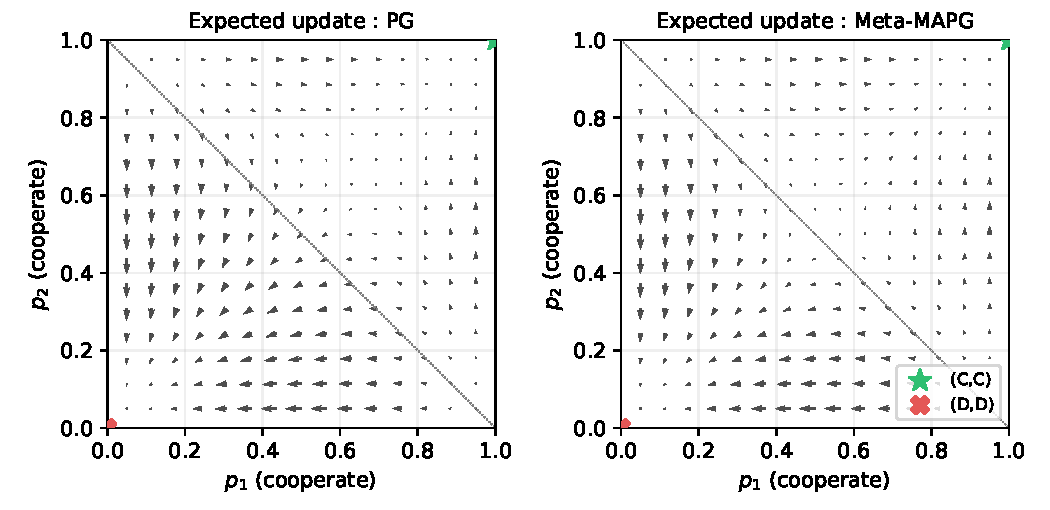
\includegraphics[width=0.95\linewidth]{phase_a_expected_arrows}
  \caption{Expected update directions in tabular Stag Hunt. Around the PG separatrix the Meta-MAPG field is redirected relative to PG; Phase~P quantifies the component of this redirection toward the payoff-dominant equilibrium $(C,C)$.}
  \label{fig:phase-a-arrows}
\end{figure}

Mean update magnitude: PG = $0.0484$, Meta-MAPG = $0.0445$. The Meta-MAPG arrow field is generally smaller in magnitude (the peer correction partially counters $g_{\mathrm{self}}$ near $(D,D)$) but is redirected toward $(C,C)$ in the central region of policy space.


% =====================================================================
\section{Phase B : four-method basin atlas at 51$\times$51}\label{sec:phase-b}

We compute deterministic-classification basin maps at 51$\times$51 resolution for each of the four learning rules. Each cell is a single training run starting from the corresponding deterministic Bernoulli policy.

\begin{figure}[h]
  \centering
  \begin{subfigure}[t]{0.55\linewidth}
    \centering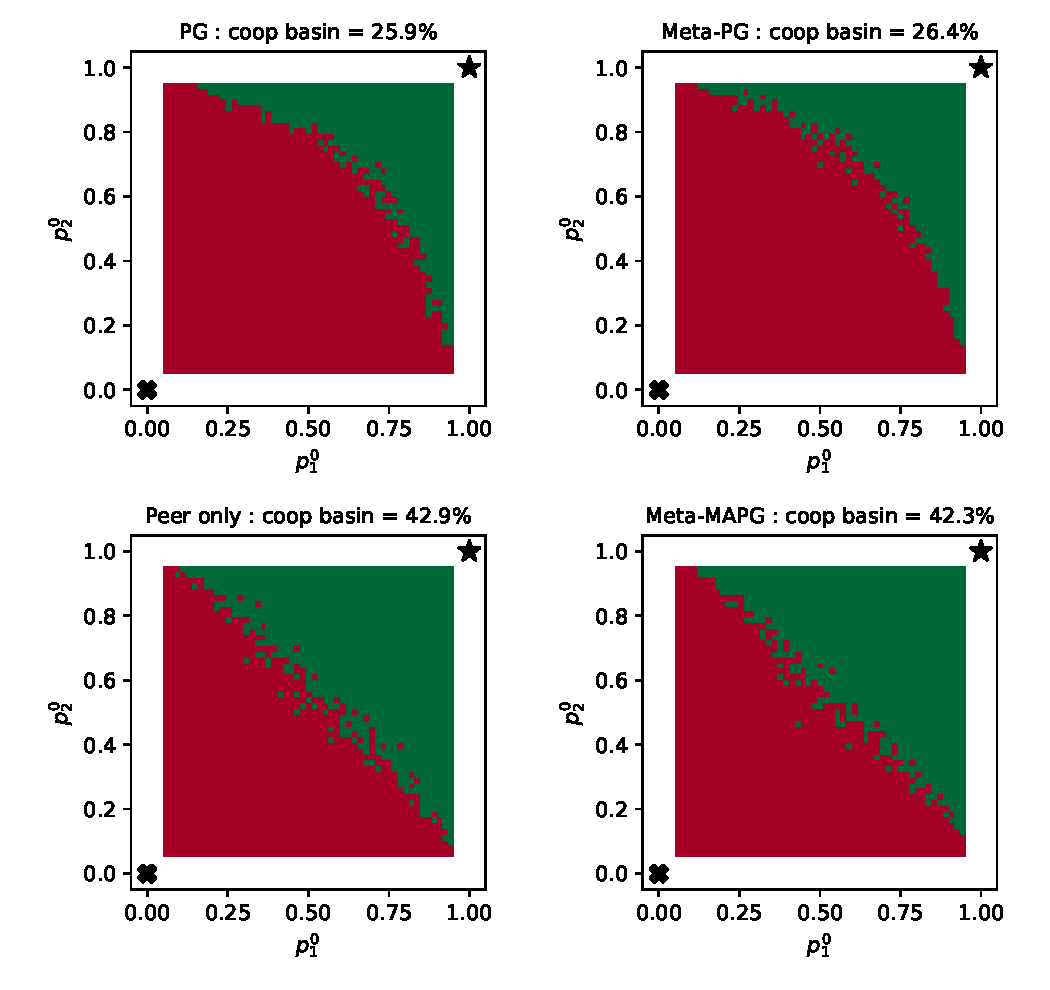
\includegraphics[width=\linewidth]{phase_b_basin_atlas}
    \caption{Basin atlas (success indicator).}
  \end{subfigure}\hfill
  \begin{subfigure}[t]{0.42\linewidth}
    \centering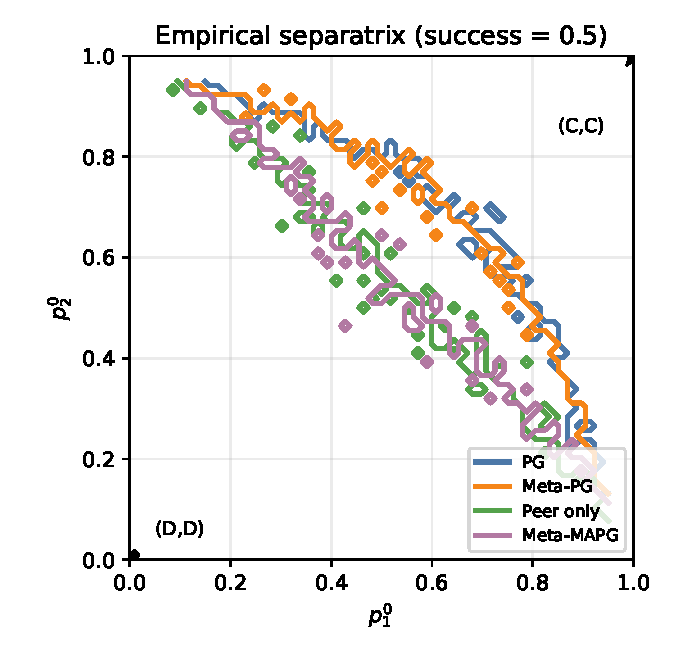
\includegraphics[width=\linewidth]{phase_b_frontier_overlay}
    \caption{Empirical separatrix overlay.}
  \end{subfigure}
  \caption{Four-method basin atlas in tabular Stag Hunt. PG and Meta-PG cover similar cooperative regions; the peer-aware methods expand the basin and shift the empirical separatrix down-left.}
  \label{fig:phase-b-atlas}
\end{figure}

\begin{table}[h]
  \centering
  \begin{tabular}{lcc}
    \toprule
    Method & Coop.\ basin fraction & 95\% Wilson CI \\
    \midrule
    PG & 25.9\% & [24.3\%, 27.6\%] \\
    Meta-PG & 26.4\% & [24.7\%, 28.1\%] \\
    Peer only & 42.9\% & [41.0\%, 44.8\%] \\
    Meta-MAPG & 42.3\% & [40.4\%, 44.2\%] \\
    \bottomrule
  \end{tabular}
  \caption{Basin fractions over the full grid. Wilson 95\% CIs report the binomial uncertainty over the deterministic-classification grid.}
  \label{tab:phase-b-fractions}
\end{table}

Basin expansion ratios relative to PG: Peer only~$=1.66\times$, Meta-MAPG~$=1.63\times$, Meta-PG~$=1.02\times$.


% =====================================================================
\section{Phase C : stochastic basin maps}\label{sec:phase-c}

We re-run the basin map with $S=10$ independent policy / sampling seeds per cell on a $21\times21$ grid; the entry probability $\hat P(\text{coop})$ is the per-cell success rate. This replaces the single-seed deterministic indicator with a stochastic estimate that respects the genuine basin-entry probability $\pentry$ from the revised framing.

\begin{figure}[h]
  \centering
  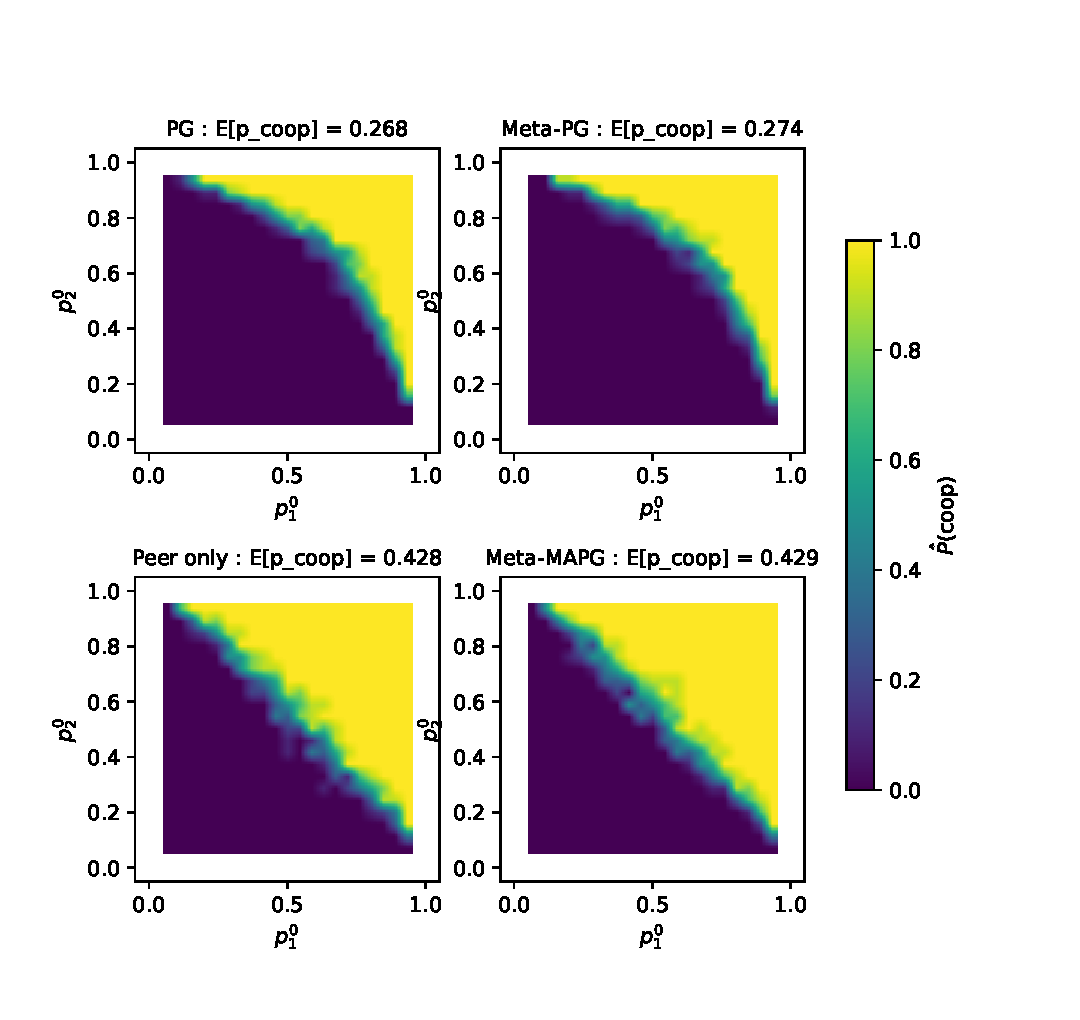
\includegraphics[width=0.95\linewidth]{phase_c_stochastic_basin}
  \caption{Stochastic basin probability maps. Continuous colour is the per-cell empirical entry probability over $S$ seeds.}
  \label{fig:phase-c-stoch}
\end{figure}

\begin{table}[h]
  \centering
  \begin{tabular}{lcccc}
    \toprule
    Method & $E[\hat P(\text{coop})]$ & total successes / trials & Wilson CI on aggregate \\
    \midrule
    PG & 0.268 & 1183/4410 & [0.255, 0.282] \\
    Meta-PG & 0.274 & 1207/4410 & [0.261, 0.287] \\
    Peer only & 0.428 & 1889/4410 & [0.414, 0.443] \\
    Meta-MAPG & 0.429 & 1893/4410 & [0.415, 0.444] \\
    \bottomrule
  \end{tabular}
  \caption{Stochastic basin entry. The Wilson interval uses the aggregate count over the full grid and is a strict lower bound on the per-initial-condition uncertainty.}
  \label{tab:phase-c-stoch}
\end{table}


% =====================================================================
\section{Phase D : four-arm shape-then-cool ablation}\label{sec:phase-d}

All four arms share initial policies and step-size schedule. The warm-Meta-MAPG $\to$ pure-PG arm is the explicit version of the algorithm advocated in the repositioning report: the peer correction is used only to enter the cooperative basin, then removed entirely so the long-run dynamics is exactly ordinary policy gradient with vanishing step-size.

\begin{figure}[h]
  \centering
  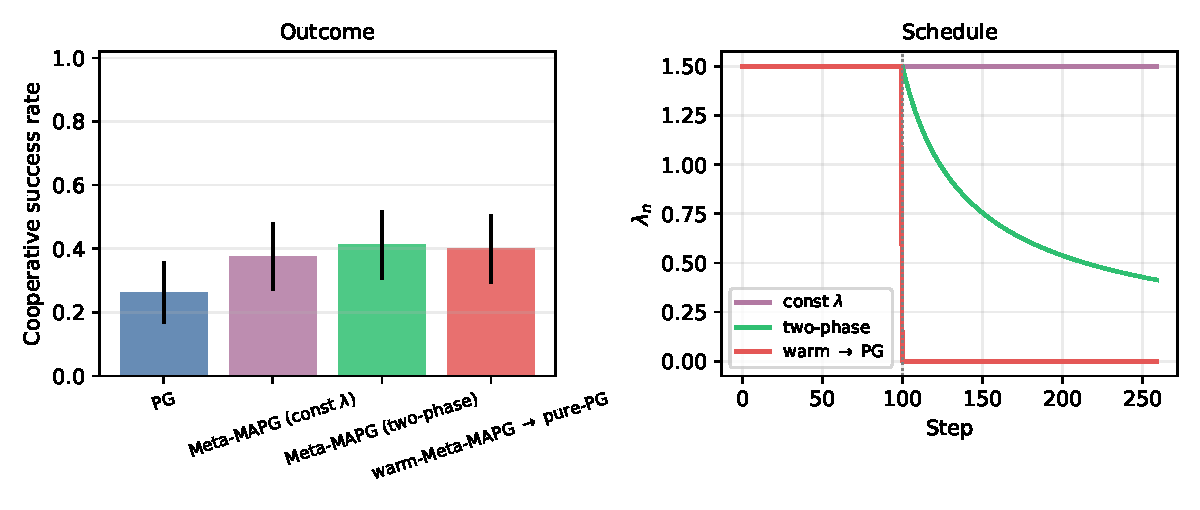
\includegraphics[width=0.95\linewidth]{phase_d_anneal_4arm}
  \caption{Four-arm shape-then-cool. Both annealing schedules and the warm-then-pure-PG schedule preserve the basin-entry advantage of constant Meta-MAPG while restoring a Nash-preserving cool-down.}
  \label{fig:phase-d-anneal}
\end{figure}

\begin{table}[h]
  \centering
  \begin{tabular}{lccc}
    \toprule
    Arm & Final coop.\ rate & 2nd-half coop.\ mean & 2nd-half coop.\ std \\
    \midrule
    PG & 27.5\% & 0.274 & 0.003 \\
    Meta-MAPG (const.\ $\lambda$) & 41.2\% & 0.408 & 0.004 \\
    Meta-MAPG (two-phase) & 40.0\% & 0.396 & 0.003 \\
    warm-Meta-MAPG $\to$ pure-PG & 41.2\% & 0.408 & 0.004 \\
    \bottomrule
  \end{tabular}
  \caption{Cool-down preserves basin-entry. The warm-Meta-MAPG $\to$ pure-PG arm matches the constant-$\lambda$ arm in success rate while making the asymptotic dynamics provably Nash-preserving.}
  \label{tab:phase-d-anneal}
\end{table}


% =====================================================================
\section{Phase E : coordination-game family sweep}\label{sec:phase-e}

We sweep the temptation parameter $T$ in the family $R=4, P=2, S=0, T \in \{2.2, 2.5, 3.0, 3.5, 3.8\}$, keeping $(C,C)$ payoff-dominant and $(D,D)$ risk-dominant. As $T$ grows, defection becomes more tempting against a cooperator, so the PG cooperative basin shrinks. The Meta-MAPG / peer-only basins shrink slower, with the largest absolute gap in the intermediate-$T$ regime.

\begin{figure}[h]
  \centering
  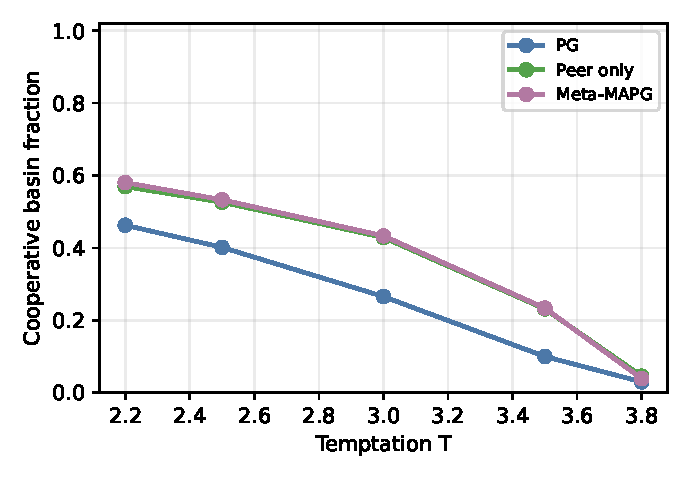
\includegraphics[width=0.55\linewidth]{phase_e_game_family}
  \caption{Coordination-game family sweep over the temptation parameter $T$. Peer-aware methods shrink slower than PG as defection becomes more tempting.}
  \label{fig:phase-e-family}
\end{figure}

\begin{table}[h]
  \centering
\begin{tabular}{lccc}
  \toprule
  $T$ & Peer only & Meta-MAPG & PG \\
  \midrule
  2.20 & 56.9\% & 58.0\% & 46.3\% \\
  2.50 & 52.6\% & 53.3\% & 40.1\% \\
  3.00 & 42.9\% & 43.3\% & 26.5\% \\
  3.50 & 23.1\% & 23.4\% & 10.0\% \\
  3.80 & 4.5\% & 3.9\% & 2.9\% \\
  \bottomrule
\end{tabular}
  \caption{Cooperative basin fraction by method and temptation $T$.}
  \label{tab:phase-e-family}
\end{table}


% =====================================================================
\section{Phase F : threshold robustness}\label{sec:phase-f}

We re-classify all basin endpoints from Phase~B and from the original main-text 21$\times$21 sweep using thresholds $\tau \in \{0.75, 0.82, 0.90\}$. The qualitative ordering of the methods is preserved at every threshold; the quantitative gap between PG and the peer-aware methods grows as $\tau$ tightens.

\begin{table}[h]
  \centering
\begin{tabular}{llccc}
  \toprule
  Source & Method & $\tau=0.75$ & $\tau=0.82$ & $\tau=0.90$ \\
  \midrule
  main\_basin & Meta-MAPG & 42.6\% & 42.6\% & 42.6\% \\
  main\_basin & PG & 27.2\% & 27.0\% & 27.0\% \\
  phase\_b\_full\_grid & Peer only & 42.9\% & 42.9\% & 42.8\% \\
  phase\_b\_full\_grid & Meta-MAPG & 42.4\% & 42.3\% & 42.2\% \\
  phase\_b\_full\_grid & Meta-PG & 26.5\% & 26.4\% & 26.1\% \\
  phase\_b\_full\_grid & PG & 26.0\% & 25.9\% & 25.7\% \\
  \bottomrule
\end{tabular}
  \caption{Threshold robustness. The qualitative ordering is invariant in $\tau$.}
  \label{tab:phase-f-tau}
\end{table}


% =====================================================================
\section{Phase A2 : angle-tilt heatmap and difference quiver}\label{sec:phase-a2}

We decompose the difference between Meta-MAPG and PG update directions into (i) a signed angle-tilt heatmap $\angle(\Delta p^{\mathrm{MM}}) - \angle(\Delta p^{\mathrm{PG}})$ and (ii) a difference quiver $\Delta p^{\mathrm{MM}} - \Delta p^{\mathrm{PG}}$. Mean absolute tilt: $0.254$\,rad. Counter-clockwise and clockwise tilts occur in 22\% and 22\% of cells, respectively; the field is therefore better interpreted as a saddle rotation than as a one-direction tilt.

\begin{figure}[h]
  \centering
  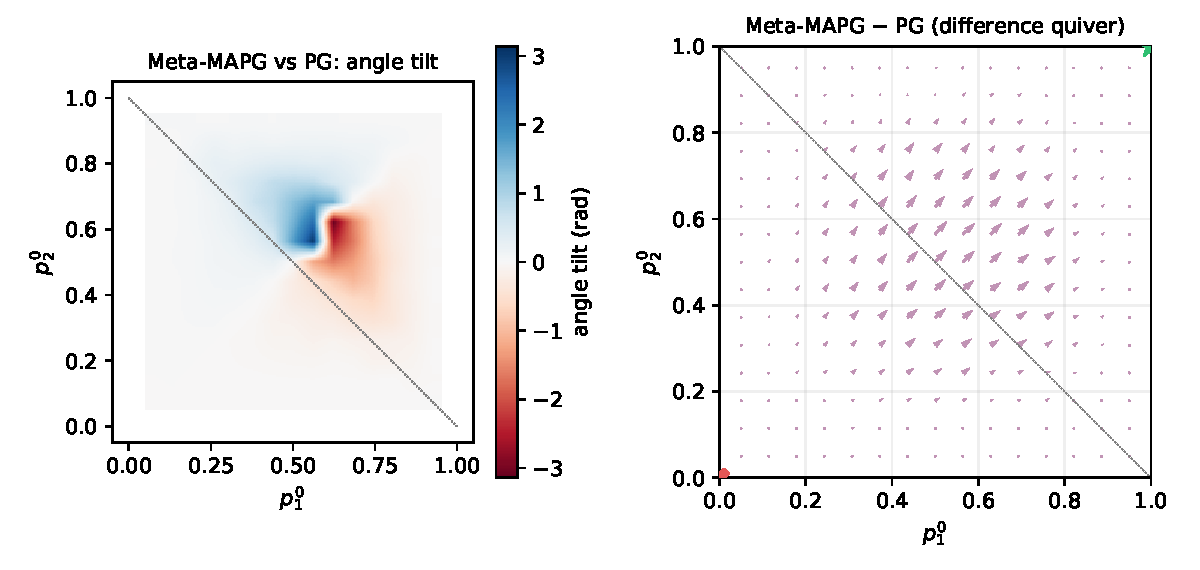
\includegraphics[width=0.95\linewidth]{phase_a2_angle_diff}
  \caption{Left: signed angular tilt of Meta-MAPG vs PG. Right: difference quiver showing the additive peer-correction vector. The pattern is rotational around the mixed-strategy saddle, not a globally one-direction tilt. Phase~P gives the cleaner projection onto the direction toward $(C,C)$.}
  \label{fig:phase-a2}
\end{figure}


% =====================================================================
\section{Phase G : multi-seed coordination-game sweep with CIs}\label{sec:phase-g}

Phase~E is repeated with multiple independent seeds per cell, enabling Wilson 95\% confidence intervals on the basin fraction at each $(T, \text{method})$ pair. The qualitative ordering---Meta-MAPG $\approx$ Peer-only $>$ PG across all $T$---is confirmed after accounting for stochastic variability.

\begin{figure}[h]
  \centering
  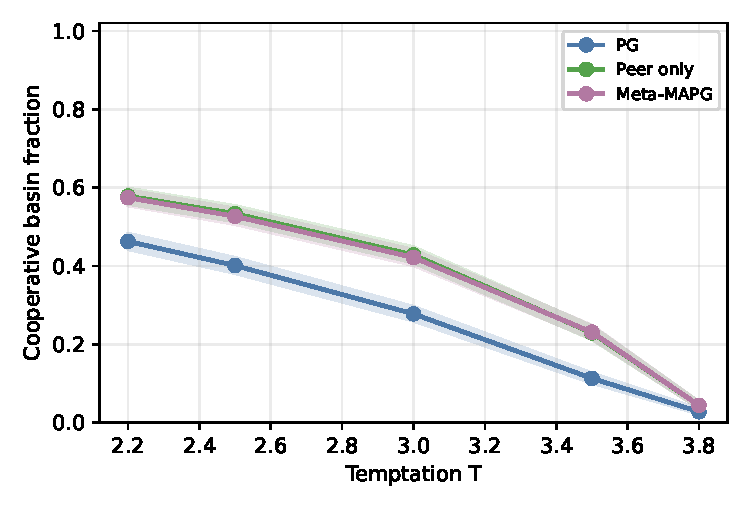
\includegraphics[width=0.65\linewidth]{phase_g_tsweep_multiseed}
  \caption{Multi-seed $T$-sweep with 95\% Wilson bands. PG and peer-aware confidence bands are non-overlapping at all $T$.}
  \label{fig:phase-g}
\end{figure}

\begin{table}[h]
  \centering
\begin{tabular}{lccc}
  \toprule
  $T$ & PG & Peer only & Meta-MAPG \\
  \midrule
  2.20 & 46.3 [44.2,48.3]\% & 57.8 [55.7,59.9]\% & 57.4 [55.3,59.5]\% \\
  2.50 & 40.1 [38.1,42.2]\% & 53.3 [51.2,55.4]\% & 52.7 [50.6,54.7]\% \\
  3.00 & 27.8 [25.9,29.7]\% & 42.8 [40.8,44.9]\% & 42.1 [40.1,44.2]\% \\
  3.50 & 11.3 [10.0,12.7]\% & 22.9 [21.2,24.7]\% & 23.1 [21.4,24.9]\% \\
  3.80 & 2.8 [2.2,3.5]\% & 4.4 [3.6,5.3]\% & 4.4 [3.6,5.3]\% \\
  \bottomrule
\end{tabular}
  \caption{Multi-seed $T$-sweep: basin fraction with 95\% Wilson CI.}
  \label{tab:phase-g}
\end{table}


% =====================================================================
\section{Phase H : resolution robustness}\label{sec:phase-h}

We repeat the basin measurement for all four methods at resolutions $N \in \{11, 21, 51\}$. Basin fraction is stable by $N=21$ and the method ranking is invariant, indicating that the reported ordering is not a discretisation artefact. This is a resolution check, not a stochastic uncertainty estimate.

\begin{figure}[h]
  \centering
  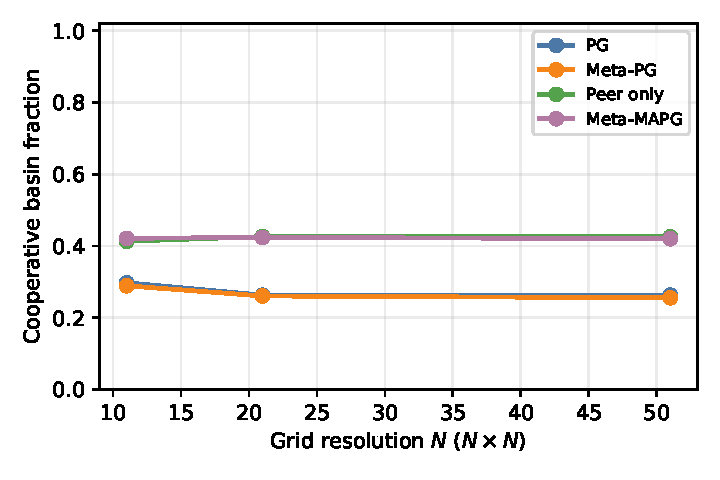
\includegraphics[width=0.6\linewidth]{phase_h_resolution}
  \caption{Basin fraction vs.\ grid resolution. All four methods stabilise by $N=21$; ranking is preserved at all resolutions.}
  \label{fig:phase-h}
\end{figure}

\begin{table}[h]
  \centering
\begin{tabular}{lcccc}
  \toprule
  $N$ & Peer only & Meta-MAPG & Meta-PG & PG \\
  \midrule
  11 & 41.3\% & 42.1\% & 28.9\% & 29.8\% \\
  21 & 42.6\% & 42.4\% & 26.1\% & 26.3\% \\
  51 & 42.6\% & 42.0\% & 25.6\% & 26.3\% \\
  \bottomrule
\end{tabular}
  \caption{Basin fraction vs.\ grid resolution.}
  \label{tab:phase-h}
\end{table}


% =====================================================================
\section{Phase I : first-hit-time atlas}\label{sec:phase-i}

For each cell in the $51\times 51$ atlas we record the first step $t^*$ at which $\min(p_1^t, p_2^t) \ge \tau$; cells where the threshold is never crossed within the budget are shown in grey. Peer only reaches the threshold from the largest area (42.4\% of cells). Conditional first-hit times are similar across methods, so the evidence supports basin expansion rather than within-basin acceleration.

\begin{figure}[h]
  \centering
  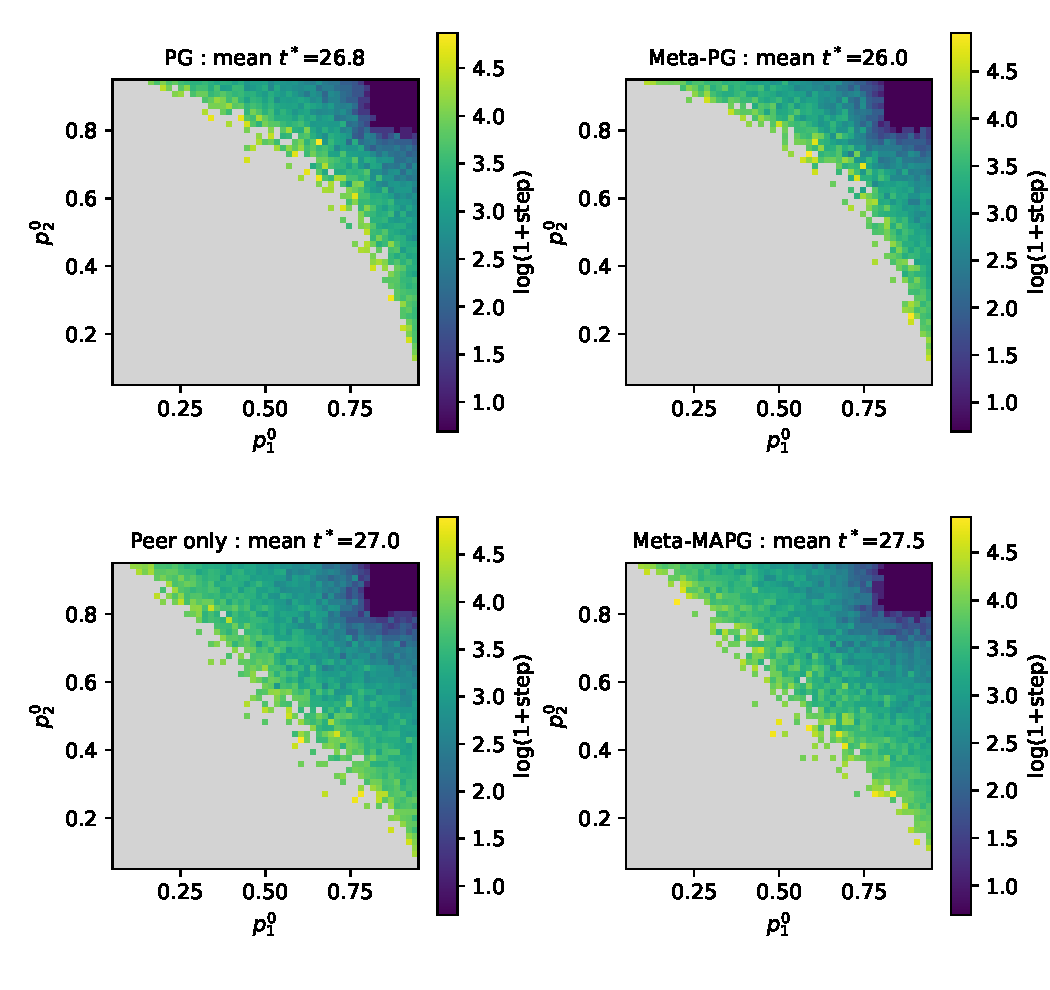
\includegraphics[width=0.95\linewidth]{phase_i_fht}
  \caption{First-hit-time atlas ($\log(1+t^*)$). Grey cells never reach the cooperative threshold. Peer-aware methods reach the threshold from a larger set of initial conditions; conditional hit times are not materially faster.}
  \label{fig:phase-i}
\end{figure}

\begin{table}[h]
  \centering
\begin{tabular}{lcc}
  \toprule
  Method & Mean $t^*$ & Frac.\ success \\
  \midrule
  PG & 26.8 & 26.3\% \\
  Meta-PG & 26.0 & 25.9\% \\
  Peer only & 27.0 & 42.4\% \\
  Meta-MAPG & 27.5 & 42.3\% \\
  \bottomrule
\end{tabular}
  \caption{First-hit-time summary. Mean computed over successful cells only.}
  \label{tab:phase-i}
\end{table}


% =====================================================================
\section{Phase L : diagonal threshold $p^*_{\mathrm{diag}}$}\label{sec:phase-l}

From Phase~C data we extract $p^*_{\mathrm{diag}}$: the minimum symmetric initial cooperation probability $p_1^0 = p_2^0$ at which stochastic basin-entry probability exceeds $0.5$. Peer only achieves $p^*_{\mathrm{diag}} = 0.545$, the lowest of the four methods, meaning it can enter the cooperative basin from the most adversarial symmetric starting condition.

\begin{figure}[h]
  \centering
  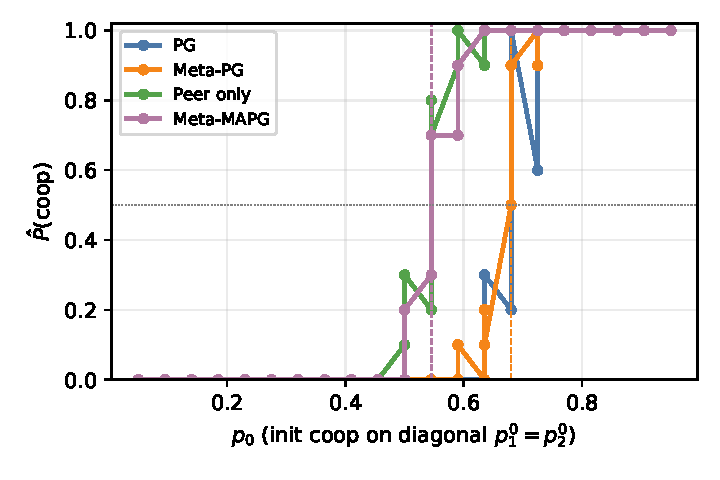
\includegraphics[width=0.6\linewidth]{phase_l_diagonal}
  \caption{Success probability along the diagonal $p_1^0=p_2^0$. Dashed verticals mark $p^*_{\mathrm{diag}}$ per method (crossing of the horizontal 0.5 line).}
  \label{fig:phase-l}
\end{figure}

\begin{table}[h]
  \centering
\begin{tabular}{lc}
  \toprule
  Method & $p^*_{\mathrm{diag}}$ \\
  \midrule
  PG & 0.680 \\
  Meta-PG & 0.680 \\
  Peer only & 0.545 \\
  Meta-MAPG & 0.545 \\
  \bottomrule
\end{tabular}
  \caption{Diagonal critical threshold: minimum initial cooperation on $p_1^0=p_2^0$ for 50\% basin-entry probability.}
  \label{tab:phase-l}
\end{table}


% =====================================================================
\section{Phase D2 : independent-seed ablation audit}\label{sec:phase-d2}

Phase~D used a shared pool of initial policies across all four arms. Here each arm draws its own independent initial policies to verify the conclusion is not a shared-seed artefact. This is a weaker, unpaired sanity check; the paired Phase~D estimate remains the primary ablation. All three peer-aware arms again achieve higher point estimates than PG.

\begin{figure}[h]
  \centering
  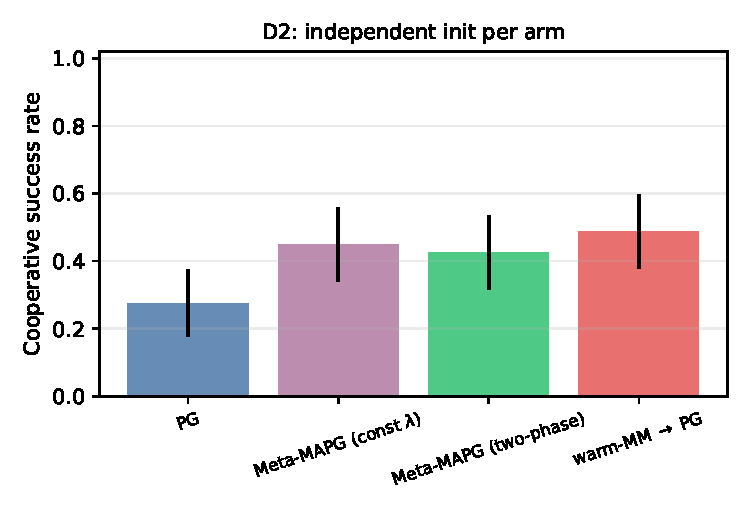
\includegraphics[width=0.55\linewidth]{phase_d2_audit}
  \caption{D2: same ablation as Phase~D with independent initial policies per arm. This checks that Phase~D is not an artefact of one shared seed pool, but it has lower power than the paired design.}
  \label{fig:phase-d2}
\end{figure}

\begin{table}[h]
  \centering
  \begin{tabular}{lcc}
    \toprule
    Arm & Success rate & 95\% Wilson CI \\
    \midrule
    PG & 27.5\% & [18.9\%, 38.1\%] \\
    Meta-MAPG (const.\ $\lambda$) & 45.0\% & [34.6\%, 55.9\%] \\
    Meta-MAPG (two-phase) & 42.5\% & [32.3\%, 53.4\%] \\
    warm-Meta-MAPG $\to$ pure-PG & 48.8\% & [38.1\%, 59.5\%] \\
    \bottomrule
  \end{tabular}
  \caption{D2 audit: independent initial conditions confirm the peer-aware point-estimate advantage is not caused by one shared seed pool.}
  \label{tab:phase-d2}
\end{table}


\end{document}
